% !TeX root = ../main.tex
% Add the above to each chapter to make compiling the PDF easier in some editors.

\chapter{Security Analysis of eSIM}\label{chapter:secAnalysis}

What this analysis wants to achieve: Analyze the eSIM architecture for potential security flaws. Reasonable attacks against the GSMA Standard

What this analysis does not include: Hardware Tampering, Assumptions that the Secure Element (eUICC) is not secure, Flaws of a particular OS or implementation

\textbf{Storyline: First, describe what an attacker could do in the system. What roles can it have, what access does it need, which assumptions can one make (i.e. dolev-yao, needs access to the network, what if the adversary switches to an internal attack (compromises an eSIM/device, then even a server, etc). What "interesting or valuable" assets are there? (keys and certificates, profile data, ...) What security goals would hinder the attacker from getting it? (CIA) \\
Then, this attacker (eve) starts attacking the network. Everything starts with the distribution of eSIM and their certificates. How are the mechanisms secured? Eve sees nothing is to gain. But once an eSIM is provisioned, maybe during the profile download? Continue to spin this story...  }

\section{Description of Model}
Recap actors, but definition should be in \ref{chapter:eSIMArch}.
\begin{itemize}
    \item Subscriber (Either actual end-user in Consumer or Device Manager in M2M 
    \item eUICC
    \item Network Operator (MNO)
    \item Provisioning Servers (SM-DP, SM-SR // SM-DP+, SM-DS)
\end{itemize}

Check System as a whole against:
\begin{itemize}
    \item Dolev-Yao (Outside) Attacker Model: Attacker can intercept, delete, change order or modify all messages sent over the communication channel between any entity. Unauthorized, external member, no/little knowledge of system, wants to compromise system or gain knowledge by logical and/or physical attacks.
    \item Inside Attacker: Compromised eSIM/Device that was previously authenticated, now malicious, and wants to download a profile/gain access etc. What happens if a Server gets compromised? Is a recovery possible?
    \item Physical Attacks are not evaluated
\end{itemize}

Then, identify security assets:
\begin{itemize}
    \item Network Access and Profile Data: How is it secured against tampering
    \begin{itemize}
        \item Network access Keys/Operator Credentials
        \item MNO OTA Keys
        \item Profile Policy File (POL1)
    \end{itemize}
    \item Management or Provisioning Commands (Start Session, Key Agreements, Enable/Disable/Delete/Download Profile, etc.): Over which channels; could they be tampered with? Most Attack Strategies focus on modifying/replaying these commands!
    \item Profile Management Data
    \begin{itemize}
        \item eUICC Keys: Where/during which transactions are these keys used, is the length sufficient, are they renewed (if yes, how)
        \begin{itemize}
            \item ISD-R
            \item ISD-P
            \item ECASD Device Key -> It must never leave the eUICC, but also won't be changed. It is only used to verify signatures or help with key-establishment
        \end{itemize}
        \item Actor Certificates and Public Keys: CI Private Root Key should obviously be hidden at all times, but what about the public certificates and keys? Are they checked by all parties properly or could an outsider reuse old/invalid certificates?
    \end{itemize}
    \item eUICC and/or Device Information: Used to identify the device. Usually public/easily obtainable information
    \begin{itemize}
        \item EIS/EID
        \item IMSI
        \item Mobile Network Dial Number
    \end{itemize}
\end{itemize}

What are the relevant interfaces, where are these assets communicated? -> Tables!

Check the interfaces and assets for protection/compliance of/with:
\begin{itemize}
    \item Confidentiality/Privacy: Concealment of Information
    \item Integrity: No improper or unauthorized change of data
    \item Availability: Services should be available at all times and function correctly -> Would only apply to actors, not to security assets -> relevant? (But DoS Attacks aim to reduce availability)
    \item Authenticity, Mutual Authentication: Entity is who she claims to be and it is allowed for her to perform the operation
    \item Parkerian Hexad would add Authentication, Possession and Utility -> Again, too much?
    \item Perfect Forward Secrecy: Keys are renewed even during a single session, ensuring that not the entire session can be decrypted if one key is cracked
    \item Freshness?
    \item Transparency?
    \item General Attacks: like Man-in-the-middle, Replay, DoS, Impersonation
    \item What if, at any point in the process, an interruption or replay of message occurs? Could the Device be forced into a dangling or even bricked state?
\end{itemize}

\textbf{Model is chosen this way because:}
\begin{itemize}
    \item Dolev-Yao is well established Attacker Model
    \item STRIDE properties do not really apply in the eSIM ecosystem
    \item CIA triad is very traditional and can be extended by other concepts \parencite{Fabian:SecReqEngin}, additionally they \textbf{do} apply in the eSIM Architecture
    \item Structural Models as described in \parencite{Fabian:SecReqEngin, Mellado:SysRevofSecReqEng} can't be applied properly as well
    \item Additionally, they mention that there is no single best model or practice, and therefore can't hold to standard
    \item Protection Profile/Common Criteria (EAL4) \parencite{SGP:05, SGP:25} is not enough, because it has it's focus on the eUICC. The ecosystem (i.e. provisioning servers) and communication is considered secure.
\end{itemize}

\section{M2M}
\subsection{Preface}
\subsection{eSIM Registration}
\subsection{Profile Download}
\subsubsection{Session Triggering SMS and ES5 Interface}
\subsubsection{Scenario \#3: Mutual Authentication}
\subsection{Profile Management}
\subsection{SM-SR Change}
\subsection{Allowance Checks}

\subsection{Structural Security Analysis}
\textbf{Some Notes:}
\begin{itemize}
    \item If SCP80 is written, both SCP80 and SCP81 can be used
    \item ES3 Interface is ignored, as it is not specified how SM-DP and SM-SR communicate with each other. However, it should be mutually authenticated and encrypted with TLSv1.2
    \item ES8 Interface is tunneled through the ES3 and ES5 Interface. Thus, encryption to these interfaces apply also to anything transported over ES8. (i.e. Data is either wrapped inside SCP80 from ES5 or TLS from ES3)
\end{itemize}

Notes on the table
\begin{itemize}
    \item T.I.: The item is sent OVER this interface
    \item U.I.: The item is used to protect this interface
    \item C: Confidentiality. The Item either cannot be read by adversaries; Or protects any underlying asset from being read
    \item I: Integrity. The Item cannot be changed unauthorized.
    \item A: Authenticity. The Item or message is sent by a trusted party and the authenticity can be checked in some form
    \item F: Freshness. The Item or message has some identifier which protects from replaying the same message
    \item E/T: Encryption or Type: By which encryption standard is this item protected or which type of channel is used
    \item PFS: Perfect Forward Secrecy. Does the channel provide PFS
\end{itemize}


\begin{table}[htpb]
  \caption[M2M Security]{M2M Security Overview}\label{tab:M2MSec}
  \centering
\begin{tabular}{m{9em}|m{.75cm}|m{.75cm}||m{.75cm}|m{.75cm}|m{.75cm}|m{.75cm}||m{1.8cm}|m{.75cm}}
     Item & T. I. & U. I. & C & I & A & F & E./T. & PFS  \\
     \hline \hline
     \multirow{2}{9em} {Network Access Keys}   & ES2 & & \cmark & \cmark & \cmark & & TLSv1.2 & \cmark \\
                                & ES8 & &  \cmark & \cmark & \cmark & & SCP03(t) & \cmark \\ \hline
     \multirow{3}{9em} {MNO OTA Keys}          & ES2 & & \cmark & \cmark & \cmark & & TLSv1.2 & \cmark \\
                                & & ES6  & \cmark & \cmark & $\sim$ & \cmark & SCP80/81 & \xmark \\
                                & ES8 & & \cmark & \cmark & \cmark & & SCP03(t) & \cmark \\ \hline
                                            
     Profile Policy File        & ES8 & & \cmark & \cmark & \cmark & \xmark & SCP03(t)  & \cmark \\ \hline 
     Profile Package            & ES8 & & \cmark & \cmark & \cmark & \cmark & SCP03(t)  & \cmark \\ \hline 
     
     \multirow{3}{9em}{Prov. Commands} & ES5 & & \cmark & \cmark & $\sim$  & \cmark & SCP80/81 & \xmark \\
     & ES3 & & \cmark & \cmark & $ \sim$ & $\sim$ & TLSv1.2 & \cmark \\
     & ES2 & & \cmark & \cmark & $ \sim$ & $\sim$ & TLSv1.2 & \cmark \\
     & ES8 & & \cmark & \cmark & \cmark & \cmark & SCP80/81 & \xmark \\\hline
     ISD-R                      & & ES5 & \cmark & \cmark & \xmark & \xmark & PSK-TLS & \xmark \\ \hline
     ISD-P                      & & ES8 & \cmark & \cmark & \cmark & \cmark & SCP80/81 & \cmark \\ \hline \hline
     Device Cert. & ES3 & & \xmark & \cmark & \cmark & \xmark & & \\ \hline
     \multirow{2}{9em} {SM-DP Cert.} & ES2 & & \xmark & \cmark & \cmark & $\sim$ &  TLSv1.2 & \cmark \\
                                     & ES8 & & & & & & & \\ \hline
     \multirow{3}{9em} {SM-SR Cert.} & ES4 & & & & & & TLSv1.2 & \cmark \\
                                     & ES5 & & & & & & SCP80/81 & $\sim$ \\ 
                                     & ES7 & & & & & & TLSv1.2 &  \\\hline
     GSMA Root Cert. & & & & & & & \\ \hline \hline
     EID/EIS & & & \xmark & \cmark & \cmark & & & \\ \hline
     IMSI & & & \xmark & \cmark & \cmark & & & \\ \hline
     
     
\end{tabular}
\end{table}

Algorithms and Key Lengths
\begin{itemize}
    \item AES 128/128 bits
    \item RSA 3072 bits
    \item ECC 256 bits
    \item Hashing for Dig.Sig., HMAC, key-derivation, RNG: SHA-256
\end{itemize}


\begin{table}[htpb]
    \caption[M2M Security by Interface]{Security by Interface}\label{tab:M2MInt}
    \centering
    \begin{tabular}{m{.75cm}|c|c}
         I & Task & Description \\ \hline
         ES1 & Register eUICC & Undefined \\
         ES2 & Profile Ordering, Management & \\
         ES3 & Initiate Profile Download \& Management through SM-SR & Undefined except for TLSv1.2\\
         ES4 & Initiate Profile Management through SM-SR & \\
         ES5 & Manage eUICC and its profiles & \\
         ES6 & Operator OTA Functionalities & \\
         ES7 & SM-SR Change & \\
         ES8 & Download Profile & \\
    \end{tabular}
\end{table}

Security Information stored on the eUICC:
\begin{itemize}
    \item eUICC Certificate
    \item Public Key allowing to verify SM-SR and SM-DP Certificates -> GSMA CI Key
\end{itemize}
Security Information stored on the SM-SR:
\begin{itemize}
    \item eUICC Certificate (via EIS)
    \item Public Key allowing to verify GSMA Certificates -> GSMA CI Key
\end{itemize}
Authentication Checks: eUICC checks Certificates of SM-SR and SM-DP via public key of GSMA-CI
    eUICC does not need to manage revocation status of SM-DP or SM-SR certificate that it receives -> Can I use outdated Certificate? Probably not since I need to establish secure channel with symmetric keys first.

\textbf{Go through profile ordering, download and enabling process again, this time with focus on security mechanisms:}

"Communication between two Security Realms [..] shall be origin authenticated, as well as integrity-protected and, unless otherwise specified [..], confidentiality protected. For all the procedures [..] the security realms are mutually authenticated [..]."

Profile Ordering is out of scope. But, operator asks SM-DP to generate profiles for an IMSI Range, provides NAAs, POL etc.

Operator performs [ES2.DownloadProfile] with SMDP, provides EID, SMSR-Id, profileType, ICCID and enableProfile. The two actors should be mutually authenticated and communication is (somehow) encrypted. The only verification the SMDP must perform, is if it is responsible for downloading and installation of the profile, but it could do more checks. \textit{A rogue operator with knowledge of the relevant input data could trigger an unauthorized profile download.} [CIAF is ensured through TLS]

SMDP retrieves EIS from specified SMSR via EID [ES3.GetEIS]. Both actors are mutually authenticated. \textit{It is not checked by the SMSR, if the SMDP is allowed to perform this operation. The SMDP must indicate, on behalf of which operator this function is performed, and when the operator matches a profile installed on the eUICC, the SMSR returns the EIS WITH the respective profile.}[CIAF is ensured through TLS]
If the EID is unknown to SMSR, an error is returned and procedure ends. If the EIS contains a profile associated with the calling SMDP, the SMDP must delete this profile before downloading a new one. \textit{Only one profile can be present by a SMDP at a time}. SMDP performs elegibility checks (is the profile compatible with the eUICC, is there enough memory left, is the eUICC certified, etc). It also verifies the ECASD ceritificate contained in EIS and extracts the public key for the further process. 

SMDP calls [ES3.CreateISDP]. SMDP checks, if it is responsible for management of this eUICC, if the target profile is not already present and if enough memory is left on the eUICC. SMSR chooses interface based on eUICC capabilites and starts session (let's assume HTTPS). Sends triggering SMS, see section \ref{sec:M2MSMS}. ISD-R creates ISD-P as requested and sends back notification to SMSR. If SMSR receives no notification, it shall trigger ISD-P deletion. \textit{Communication between SMSR and ISD-R is over CAT-TP or HTTPS. If CAT-TP, it's SCP80 and symmetric keys. If HTTPS, it's PSK-TLS encrypted. Authenticity of SMSR is not checked by eUICC, but the assumption underlies, that only the correct SMSR knows the symmetric key. SCP80/81 ensures Integrity and Confidentiality. However, PFS is never achieved as the pre-shared key is always the same and the session key is directly derived from it. As ciphersuites TLS\_PSK\_WITH\_AES\_128\_GCM\_SHA256 \& TLS\_PSK\_WITH\_AES\_128\_CBC\_SHA256 are used, which are even considered weak by current standards.}

For the profile download, a secure SCP03t channel is used. For this channel, new keys have to be established between ISD-P and SMDP. As establishment protocol, ECKA ElGamal is used. SMDP starts communication with SMSR, within [ES3]SendData function the [ES8]EstablishISDPKeySet function is contained. SMSR performs its checks (responsibility for target eUICC, ISD-P is already created, Commands from SMDP are allowed to be executed by ISD-R). \textit{The check, that the SMDP is allowed to perform this operation and the integrity of the message relies on the Mutual Authentication on ES3}. If not already open, the SMSR starts a Session with eUICC \ref{sec:M2MSMS} and sends the ES8 command within the ES5 channel (in case of HTTPS via POST/response). ISDP verifies (via ECASD) the SMDP Certificate. \textit{The ECASD holds only the GSMA CI Public Key. This key is used to verifiy the received certificate. However, since the eUICC may not know the current time and DOES not know of any certificate revocation, the certificate may be outdated or revoked, but the verification still succeeds. Then again, the certificate in question should have already been checked previously by the SMSR before initiating communication with SMDP.} 
ECASD extracts and stores public key and generates a 16 or 32 byte Random Challenge. The challenge (or any error) is sent back to SMSR and SMDP. SMDP then generates an ephemeral key pair, signs the RC with its private key. Within the ES3 and ES5 channel, the ES8 command is sent including the signed challenge, the ephemeral public key and a signature of both. ECASD checks the received information and calculates a shared secret (ShS). The ShS is returned to the ISD-P, which derives the AES128 keyset from it, and sends a receipt to the SMDP. SMDP also calculates ShS and Keyset. The session key agreement protocol is verified to be secure in \parencite{Ding:FormAnalSessionKey}. \textit{The eUICC certificate or public key is never sent to the SMDP by the eUICC itself. The SMDP relies on the information inside the EIS provided by the SMSR. If this information is faulty, the key establishment will never succeed. -> Why not directly send certificate from eUICC?} 
In case any error or timeout of messages occurs, a special error-handling subroutine occurs, where the SMDP must delete the created ISD-P. If this error routine again fails, the SMDP will get the chance to delete the ISD-P on the next profile download procedure.

Profile Download is again initiated by SMDP via the [ES3]SendData containing the profile data. SMSR verifies (again) that request from SMDP is acceptable. \textit{Same checks as in the step before, with the same thoughts.}
SMSR forwards the profile package to eUICC. ISD-P must verify the security of the profile package. 
The profile package is secured by SCP03t. SCP03t functions the same as SCP03 \parencite{GPC:AmendE}, but adds two commands for the secure channel initiation. However, two different keysets can be used: Either the previously established keys, or the SMDP chooses random keys. If the latter option, the SMDP must exchange the keys used on the eUICC by encrypting the random keys with the ISD-P keyset and sending them through the ES8 channel. These new keys are then used instead for securing the SCP03t channel. An "advantage" is, that the SMDP can encrypt the profile package before knowing the session keys of the eUICC. \textit{SCP03t secures the confidentiality, integrity and authenticity of the profile package. It uses AES-CBC and an encrypt-then-MAC for integrity protection. Authenticity is guaranteed by the previous mutual authentication between SMDP and eUICC. It also protects against replay and out-of-order attacks, and other strong notions of security, as proven in \parencite{Sabt:CryptanGPSCP}. The whole profile package is seen as a transparent block of data and encrypted as such, even if the data is too long to be sent in a single, 1024 Byte package. It should also ensure PFS, since a new session key is used every time.}

The SMDP may need to call the SendData function several times, depending on the profile package size. If all commands return successfully, the SMDP calls the [ES3]ProfileDownloadCompleted to indicate to the SMSR the profile download is complete. The EID of the eUICC and ICCID of the profile function as identifier, such that it is not possible to call the function if the named profile/ISD-P was previously not created. SMSR updates the corresponding EIS if all checks pass and sets the profile state to "disabled". If during the profile download any error occurs, the same error-management procedure as above applies (deletion of ISD-P), unless the POL1 of the installed profile prohibits the deletion (i.e. profile has fallback or emergency attribute set), then the SM-DP assumes that the profile download was successful.
\textit{The spec is ambiguous to what happens to the SCP03 keyset:} In the procedure of section 3.1.3, the session keys/random keys MAY be deleted from the eUICC, but in section 4.1.3.3 (and the definition of SCP03t) the keys SHALL be deleted after the profile download. Section 3.1.3 also allows a retention of the keys on the SMDP or a handover of them to the operator. However, if the keys are deleted on the eUICC, a storage in any form is worthless.

The procedure may end here with the SMDP sending a the [ES2]ProfileDownload response to the operator about a successful download. The SMSR also sends a notification to the M2M-SP which may be directly over the ES4 interface or again over the SMDP [ES3/ES2]. \textit{If these notifications/function calls are blocked, nothing bad inherently happens. The SMDP and SMSR both know, that the profile is successfully downloaded, and the eUICC has a valid profile installed. If the operator does not receive any notification, he may assume the function call expired. Then, he can either call the function again, where the SMDP quickly finds out about the already installed profile. The other option is to audit the EIS (through SMDP or SMSR) and again find out about the already installed profile. In any case, the eUICC is able to connect to the network and function correctly, if the target profile was to be enabled.}

The profile may be enabled directly after the profile download or at any later point in time. The enabling may be triggered by the operator directly on [ES4] or through the SMDP.
The SMSR must verify, that the request (by Operator or SMDP) is acceptable (responsibility, profile with ICCID is installed and disabled, POL2 of currently enabled and target profile allow enabling, operator is allowed to perform enabling).
SMSR starts communicating with ISD-R (e.g. over SMS) and sends the [ES5]StoreData command with the request for profile enabling. ISD-R checks POL1 of the currently enabled profile (if profile is allowed to be disabled). If POL1 allows, the ISD-R disables the current ISD-P and enables the target ISD-P. The ISD-R sends a response SMS to the SMSR, indicating if the enabling was successful and the device performs a refresh (reboot). 
The device will try to attach to the new network using the NAAs of the new profile. The ISD-R will again try to send a SMS notification to the SMSR and waits for a confirmation [ES5]HandleNotificationConfirmation from the SMSR. If sending the SMS fails \textit{after a unspecified number of retries} or no confirmation is received, the eUICC considers this as an error (no network connectivity), disables the new profile and re-enables the old profile. As soon as the confirmation of SMSR is received, the ISD-R considers this as a successful attachment and will no longer try to disable the new one.
The ISD-R checks again the POL1 of the old profile. If it should be deleted when disabled, ISD-R will enforce the policy, unless the old ISD-P has the fallback attribute set. The information about deletion is sent within the response to the [ES5]HandleNotificationConfirmation command. SMSR checks then its POL2 on the old profile and may enforce an ISD-P deletion, if not already done (and the eUICC can deny it, if the POL1 does not allow deletion).
SMSR will update the EIS accordingly (new profile enabled, old profile disabled or deleted) and send notifications to all relevant parties (M2M SP, SMDP, Operator of new and old profile). \textit{CIAF is protected by the secure channel between SMSR and eUICC (SCP80 in case of SMS and CAT-TP, PSK-TLS if HTTPS commands are used). One could block the attachment SMS, such that the eUICC triggers the re-enabling of the old profile. However, the device then still has a working network connection and SMSR may try the profile download again. Can't criticize the standard, as this fallback is a better option than leaving the device in an unreliable detached state. Blocking any confirmation notifications would give the same results as above, either the operator may try again or audit the SMSR.}

Profile Disabling and ISD-P deletion (triggered on ES4 or ES2) requires the same steps and checks as done above during the download and enabling process. An enabled ISD-P can never be deleted, it has to be disabled first. However, if the call is to delete the ISD-P, the SMSR will automatically disable it. Fallback-Attributes, POL1 or POL2 can block the operation. The communication to the eUICC is exclusively over the secure ES5 channel.

SM-SR Change: It is possible to change the responsible SMSR. The SM-SR change must be "allowed" and all parties must have their certificates signed by the CI. The initator (e.g. Operator) calls [ES4]SMSRChange function to the new SM-SR. The Initiator must only provide the EID and current SMSR-ID to the new SMSR. It is assumed that they are mutually authenticated. New SMSR [nSMSR] checks, if the change is acceptable. The initiator calls then the [ES4]SMSRChange function, containing only the relevant EID and target-SMSR-ID. The old SMSR [oSMSR] can only deny the request, if there is any pending action for the target eUICC or the function requestor (operator) is not allowed to manage the eUICC. \textit{This procedure does not seem well tested. Only the initiator is checked, if the request is acceptable. It should be acceptable, as soon as the operator has a profile installed on the eUICC, or the M2M-SP is allowed via a PLMA. Having a rogue (but valid) SMSR and getting the operator somehow to request the change, all the eUICCs will be transferred to the new SMSR without the old SMSR ever checking (e.g. with the M2M-SP) if this is actually wanted. (i.e. the checks only test, if the NEW SMSR wants the change, not the old one). Then, the new SMSR can just delete the profiles on the eUICC and all attached devices are dead. \textbf{How would i get the operator to request the change? Can an attacker impersonate?}} 
oSMSR then calls the [ES7]HandoverEUICC function which triggers the verification by nSMSR. The complete EIS is sent to nSMSR, which validates the ECASD certificate and extracts the public key. In return, nSMSR calls the function [ES7]AuthenticateSMSR, such that the oSMSR can trigger the key-establishment process with the ISD-R. This key-establishment is the same as the one between SM-DP and ISD-P, but instead of SM-DP the nSMSR is used and ISD-R instead of ISD-P. oSMSR still acts as a transport tunnel until the new keyset is created. If at any point during this process a function timeout or any other error occurs, the oSMSR must cancel the procedure and send "failed" as a result to the [ES4]SMSRChange function. Both the eUICC and oSMSR then remain in the state as before the change was initiated. As soon as the nSMSR has established a new keyset with ISD-R (success response to [ES5]EstablishISDRKeyset), both SMSRs consider the hand-over as successful, but maybe with a warning if any of the remaining steps do not fully complete. Since nSMSR now has a keyset directly with the eUICC, it opens a secure channel and calls the [ES5]FinaliseISDRHandover, which deletes the keys of oSMSR. \textit{The entire security of this process relies on the fact, that the initiator is valid and the new SMSR has a certificate issued by the GSMA-CI. A compromised operator (with a profile installed on the device) could easily trigger this process without the M2M-SP (the owner of the eUICC and probably attached device) being able to stop this. MITM should not be possible due to the certificates and authenticity checks. Security between SMSRs is unspecified, but probably TLS. Security on ES5 is again SCP80/81.} As soon as nSMSR sends the response of [ES7]HandoverEUICC to oSMSR (either success or success with warning), oSMSR deletes the EIS for the target eUICC. oSMSR sends a notification to the initiator about a successful handover, and nSMSR sends notifications to all operators owning profiles on the eUICC. \textit{At that point, operators can only disable profiles on the eUICC if the change was not valid. However, the eUICC is in control of the nSMSR - which could then delete all profiles and therefore disable any network connection of the device.}

Master Delete: Functionality to delete any profile without the fallback-attribute, even if POL1 or POL2 would forbid it.
Undefined function call from Initiator containing EID and ICCID to SM-SR. SM-SR then asks relevant SM-DP for authorization (again unspecified), which again asks Operator for authorization. If any response fails or contains "not allowed", the SM-SR is not allowed to execute the function. \textit{If confirmation message is blocked, SM-DP or SM-SR must assume that it is not allowed. Therefore blocking the message would deny a valid deletion process.} Otherwise, a delete token is returned to the SM-SR. SM-SR sends [ES5]MasterDelete command to ISD-R via an MT-SMS including the Delete-Token (The Delete Token is a Delete Command with a signature created with the AES-Key with key-version '70' and identifier '01' \textbf{NEVER mentioned elsewhere in the spec, where this key comes from, how it is established}, defined in \parencite{GPC:CardSpec} Section C.4.6. The Token shall be usable only once.) \textit{The message is secured by SCP80. Integrity and authenticity of the DELETE command is additionally ensured via the signature through the AES key.} If the verification of the token by the ISD-P is successful, the ISD-R deletes the target ISD-P and profile, and sends an MO-SMS to the SM-SR. SM-SR updates the EIS accordingly.


\subsection{Session Triggering SMS}\label{sec:M2MSMS}
All (HTTPS) sessions start with an SMS sent by the SM-SR. This SMS is addressed to the ISD-R and is defined in ETSI TS 102 226 \parencite{TS102:226}. The exact format must comply with the "Administration Session Triggering Parameters" as defined in GlobalPlatform Card Specification Amendment B \parencite{GPC:AmendB}.
The SMS triggers a HTTPS Session, where the Pre-Shared Key of the ISD-R is used for a PSK-TLS Handshake. The following communication for commands sent through the ES5 Interface (SM-SR <-> ISD-R) is then secured via this session key and the underlying protocol is SCP80 or SCP81.
The Triggering-SMS may contain the address of the SM-SR for connection or parameters for DNS-Resolution. If the payload of the SMS is empty, the ISD-R connects to the default (stored) SM-SR address. 
\begin{figure}
    \centering
    \begin{minipage}{0.5\textwidth}
        \centering
        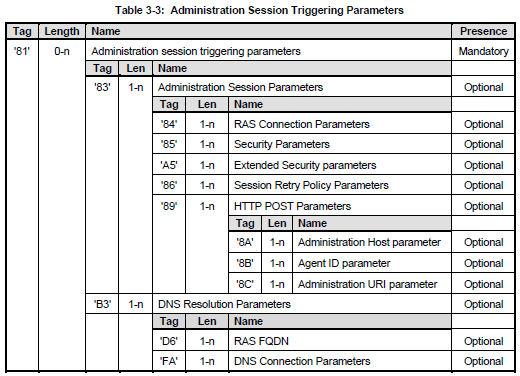
\includegraphics[width=0.9\textwidth]{pictures/adminSessTrigParam.png} % first figure itself
        \caption{Admin Session Triggering Parameters \parencite{GPC:AmendB}}
    \end{minipage}\hfill
    \begin{minipage}{0.5\textwidth}
        \centering
        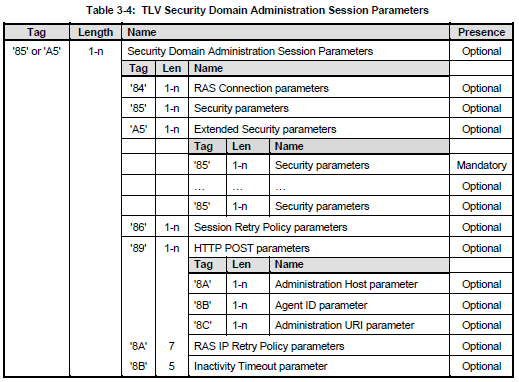
\includegraphics[width=0.9\textwidth]{pictures/secDomAdminSessParam.png} % second figure itself
        \caption{Security Parameters contained within Admin Session \parencite{GPC:AmendB}}
    \end{minipage}
    \label{fig:APDUStruc}
\end{figure}
However, it is not clear from the specification, if the triggering-SMS does already contain encrypted payload. The only possible encryption is via the pre-shared ISD-R key.

The Question and Attack Idea is: If the Session-triggering-SMS is in plain and only conforms to the standard, could such an SMS be easily crafted and sent to the eUICC, such that it is "forced" to connect to an (not existing) SM-SR? This would deplete the battery of the M2M-device and/or consume processing resources while the device tries to connect.

If the Session-triggering-SMS is in fact encrypted and the data cannnot be modified, could the SMS be replayed several times to force the eUICC to connect to the (valid) SM-SR, even though no profile operation is intended (again, DoS type of attack)

\textbf{Steps so far:}

In a trace taken from a successful profile download and a profile switch, the header of the SMS is easily readable and contains basic information (about message origin, timestamp, etc.). 
\begin{figure}
    \centering
    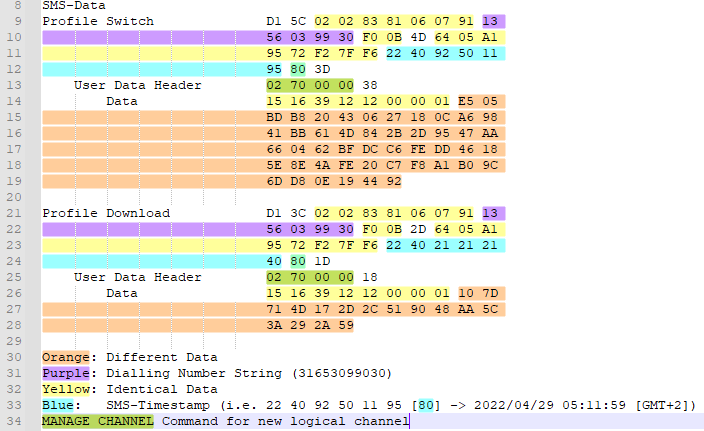
\includegraphics[width=.75\textwidth]{pictures/SMS_trace.png}
    \caption{Comparison of SMS Envelope Data for Profile Switch and Download}
    \label{fig:APDUDat}
\end{figure}
The user data of the SMS-envelope contains again an identical header (02 70 00 00 is a MANAGE CHANNEL Command for a new logical channel -> hint that it's the correct SMS), but the data looks scrambled (encrypted?) and does not match any of the specifications fully.

Try to match the command header to the TS 102 225 \parencite{TS102:225} -> 2 Bytes too much, Padding Counter (PDCNTR) does not add up, GPC Amendment B \parencite{GPC:AmendB} structure is completely ignored.

Then, in GPC \parencite{GPC:AmendB}, section 3.3.1.1, "The SD shall set up a TCP connection with the RAS IP address and then establish secure communications using its own PSK TLS key (see section 3.3.2). The SD shall resolve all the parameters needed to establish this connection and to manage its security from the triggering message and/or the parameters stored by the
SD/ISD (see sections 3.7 and 3.8).", which would state that the triggering SMS must be unsecured and \textbf{then} the channel will be secured by TLS.

Is the SMS/Data as seen in \ref{fig:APDUDat} the wrong one? The further trace \textit{looks} like its over TCP/IP (and thus HTTPS).

In the 102 225 \parencite{TS102:225} there is a note that the counter, padding counter and checksum are also encrypted, i.e. 10 7D [...] 2A 59 in the download SMS must be encrypted data. This would also fit with the fact that AES-CBC with a 128bit key is used, because the data is 16 bytes long (exactly one block). With the Profile-Switch SMS it is 48 bytes, so 3 blocks. This would also solve the problem with the counter (that the number is much too high and seemingly random).
The header coincidentally matches exactly with the header of the 102 225, as shown in the excel sheet. On page 36/37 in SGP02 it also says that SPI1=16 and SPI2=39. The only thing I still don't understand is the 15 at the beginning, that must be either CPI or CHI, but I can't find in any spec where that should be defined.
The length of the checksum must be 32 or 64 bits according to the spec, I think that only 32 bits are used, otherwise the download SMS is too short (with 64 bits only 2 bytes of possible data would be left).

The communication takes place between the server (SM-SR) and the associated applet (ISD-R) on the eUICC. Both have a previously exchanged AES key, which is the same for each new connection setup and min. 128 bit long.
The SM-SR sends the SMS to the eUICC, consisting of SMS header (in plaintext), and SMS data. The data then contains the actual command that the eUICC should establish a connection to the SM-SR (see screenshot).  
The encryption used is AES in CBC mode (128 bit key and block size). The IV is 0 \parencite{TS102:225}. 
 
The encrypted data then contains: 5 byte counter, 1 byte padding, 8 byte CC (AES-CMAC) and the "Session Triggering Parameters". The CC is calculated over all bytes of the "User Data" in the SMS, thus also over the counter. I.e. a bit flip attack should not be possible so simply, since I must hit not only with the counter correctly, but also with the CC.
If in general an attack on this AES version should not be possible, as described in \url{https://crypto.stackexchange.com/questions/47328/is-cbc-mode-with-a-fixed-iv-secure-if-a-counter-is-prepended-to-the-plaintext}, where it is proven that "nonce-based CBC" is comparably secure as "standard CBC", as long as the first cipher block is unique - which is actually guaranteed by the ever increasing message counter. 
Padding Oracle Attacks should not be possible, as the counter is encrypted and within the checksum calculation.

\subsection{Allowance Checks}
It is (almost) never checked, if the function requester is allowed to perform the function, as long as the provided certificate (issued by GSMA) and function input is correct.

Construct an environment, where either a SM-DP or Operator are malicious but with a valid, GSMA-issued certificate for their respective roles. Both must run through the GSMA certification schemes. However, a governmental agency could definitely achieve this and then perform the malicious operations until the certificates get revoked.

A operator could perform almost any task when knowing the EID of a target eUICC and the address of the relevant SM-SR/SM-DP. It all should start with a profile download. The servers never check, if the operator is actually allowed to request the profile download. Once a profile is downloaded on the eUICC, the operator is allowed to manage this profile and could "lock" the eUICC via the profile policy POL1 by setting it to "must not be disabled" and "must not be deleted". It could also trigger an SM-SR change (with a second, controlled SM-SR) and completely gain control of the target eSIM.

\textbf{Elaborate on the possibilities, compare it to SS7 attacks! Certification is currently only possible by GSMA, but \textit{if/when} the eSIM-System is as popular and well-established as GSMA imagines, a single CI is probably too risky and complicated (see consumer version), which leads to other authorities being able to certify (Business Growth leads to more authorities leads to more risks and chances of involvement of dishonest parties).}

\subsection{Other Attack Ideas:}
\begin{itemize}
    \item No PFS Enforced for SM-SR <-> eUICC Communication. Used ciphersuites TLS\_PSK\_WITH\_AES\_128\_GCM\_SHA256 \& TLS\_PSK\_WITH\_AES\_128\_CBC\_SHA256 for the PSK are classified as "weak" -> usage of ephemeral keys for session initiation could be recommended. However, TLS\_PSK\_WITH\_AES\_128\_CBC\_SHA256 is still recommended in GPC\_SPE\_011.
    \item \url{https://www.ietf.org/id/draft-ietf-tls-external-psk-guidance-06.html} recommends a key-establishment process (psk\_dh) for PSK-TLS
	\item Why are symmetric preshared keys needed? If the device needs to verify the SM-SR/SM-DP Certificates anyway, then why use PSK before
    \item Why do we need separate SM-SR and SM-DP
    \item How does eUICC check certificate validity? (without any real time or revocation reference)
    \item M2M is EAL4 tested
    \item Update SCP03 to SCP10? Probably not (https://tches.iacr.org/index.php/TCHES/article/view/8588/8155)
    \item Compromised SM-SR leads to all related devices being lost/compromised -> Single point of failure
    \item In theory, it should be possible to hijack communication between SM-DP and SM-SR iff:
    \begin{itemize}
        \item Attacker has cracked SM-SR certificate and private key
        \item SM-SR Certificate is revoked
        \item Operator decides to perform management operation through this SM-SR nonetheless. Asks SM-DP to start communication with SM-SR through specified address
        \item SM-DP shall not refuse to perform the operation as specified in Spec
        \item Attacker reroutes communication to its server, impersonates SM-SR, starts handshake etc. with SM-DP
        \item No further action can be performed other than denying the service, as the ISD-R keys are not known to the attacker 
    \end{itemize}
\end{itemize}



\section{Consumer}
\begin{itemize}
    \item MitM should be possible? 
    \item SIM Profile Cloning as described in \parencite{Ahmed:TransparancyProfile}
    \item What if "successful download notification" is never received (SM-DP+ has retry counter before profile package is marked invalid, but max value is not specified) -> Download of same profile for multiple devices with same Activation Code
\end{itemize}

\subsection{Attacker Model}
The attacker model changes in the consumer version slightly. In the M2M-Spec, the attacker only wants to attack the eSIM service, such that eSIM does not have connectivity anymore (i.e. alteration of profile, DoS, battery exhaustion, etc). In the consumer spec, the attacker may not only want to deny the network connectivity (i.e. harm the user), but the attacker may also be a consumer, who wants to take advantage of the profile provider (i.e. use profile on multiple devices even if not allowed, gain more data volume, etc). 

What could a malicious LPA do?

\subsection{Structural Security Analysis}

\subsubsection{Prefacing Security Considerations}
Any of the remote secure communication for RSP must be:
\begin{itemize}
    \item mutually authenticated: The client first authenticates server and then server authenticates client (via certificates issued by GSMA). However, client authentication does not apply to LPA, only to eUICC
    \item private: eUICC must not reveal any private data to an unauthenticated server or generate any signed material before authentication
    \item protected: A common cryptographic suite must be negotiated and session keys must be generated using PFS.
    \item authorized: Server must always check if the requesting client is authorized.
\end{itemize}

Profile is protected by SCP11a \parencite{GPC:AmendF} with slight modifications: signatures based on ECDH keys are used to authenticate to the other side instead of static key pairs. MACing and encryption is done as specified for SCP03t.

\begin{itemize}
    \item SCP11a: Key Agreement Scheme based on certificates, used to generate session keys. Provides PFS due to ephemeral key pairs generated by server and device.
    \item SCP03(t): Symmetric Encryption Protocol, uses the session keys generated by SCP11a. Ensures Integrity and Data Confidentiality
\end{itemize}

TLSv1.2 is used as minimal version for all RSP connections. Cipher suites are TLS\_ECDHE\_ECDSA\_WITH\_AES\_128\_GCM\_SHA256 and TLS\_ECDHE\_ECDSA\_WITH\_AES\_128\_CBC\_SHA256 \textit{GCM version is "recommended", "CBC" is considered weak (on the basis of tricky CBC implementations often providing security holes).}

ES2+, ES9+, ES11, ES12 and ES15 use HTTP and TLS as transport layer to communicate. ES2+, ES12 and ES15 use TLS with mutual authentication, ES9+ and ES11 use server authentication where the LPA is always the client. Integrity, Confidentiality and Authenticity of each message is left to TLS. 

All functions are executed in a Request-Response functionality, as defined in \parencite{SGP:02}. However, in contrast to the M2M version, functions are not assigned a "Validity Period". A replay of messages or a second function call is handled by the respective functions, who are supposed to do either nothing or the defined functionality.

Each server (SM-DP+ and SM-DS) has up to three certificates: 
\begin{itemize}
    \item CERT.XXauth.ECDSA: Certificate to authenticate the Server (XX) to the eUICC
    \item CERT.DPpb.ECDSA: Certificate of SM-DP+ for profile package binding, this certificate is used for key-establishment 
    \item CERT.XX.TLS: Certificate for TLS Session Establishment
\end{itemize}

\subsubsection{Profile Ordering and Download Initiation}
Contract Subscription Process is only informative in the Spec. End User concludes a contract with MNO. EID and IMEI of the target device may be provided and related device capabilities may be acquired. If so, the operator can verify, if the device (and eUICC) is supported and could already generate a specific profile type. However, no security considerations here, since this is a proprietary process similar to a normal SIM.
The download preparation process is between Operator and SM-DP+. [ES2+]DownloadOrder needs as input data either the ICCID of the target profile and/or a profile type. The EID is optional, but should be provided if either the default SM-DP+ or SM-DS is used for download. SM-DP+ reserves an ICCID (identical to the one provided) and generates or chooses a profile according to the provided type. Already at this stage, the profile package is "protected", the profile package TLV is split into several, 1020 bytes long encrypted and MACed packages. The enc\&MAC follows the SCP03t specification. The keys for this are either random and attached to the profile package, or session keys already agreed on with the eUICC. \textit{The spec in section 2.5.3 allows both options, however following the profile download procedure, it is not possible to use the session keys for profile protection, because at this stage the SM-DP+ never had any previous communication with the eUICC (and session keys must not be stored nor reused!).} The ICCID is returned to the operator. If needed (for SM-DS and AC provisioning) a matching-ID is generated by the operator - but this can also be done by the SM-DP+ in the next step. 

A few words on the topic "Matching-ID" (M-ID): It is a mandatory information for the profile download process, but may be zero-length when used in combination with the default SM-DP+. The M-ID consists of upper-case, alphanumeric characters (0-9, A-Z) and "-" in any combination. It is generated during the download initiation procedure, either by SM-DP+ or by the operator, but is known by both. If it is not zero-length, the M-ID represents a unique identifier to match a profile download order, and the SM-DP+ must only accept profile download requests who provide a valid M-ID. \textit{The activation code contains only readable/plain-text information (SM-DP+ Address, Matching-ID). One could generate random M-IDs and try to download a "released" and unpersonalized profile that happens to match the M-ID.} 

Operator calls [ES2+]ConfirmOrder. If the EID has not been provided before and the default SM-DP+ or SM-DS is used for profile download, it must be sent as an input to this function. SM-DP+ confirms ICCID allocation, generates M-ID if not provided by operator and store M-ID and EID. If a confirmation code is needed for profile installation, a SHA256 Hash is calculated of the CC and stored alongside the M-ID. A release flag is a required input, which identifies if the profile should be immediately released for profile download. The SM-DP+ returns an indication about the state of the profile and successful execution.
\textit{CIA on the ES2+ interface for these function is provided by TLS: The parties must be mutually authenticated through the GSMA-CI signed certificates and negotiate a session key for the communication. Session Replay is also handled via TLS, and even if, the SM-DP+ functions handle an additional execution gracefully and the profile state is left unchanged.}

\subsubsection{Common Mutual Authentication Procedure}
This Mutual Authentication Procedure is used for authenticating the eUICC to either the SM-DP+ or SM-DS. 
\begin{figure}
    \centering
    %\includesvg[width=\textwidth]{pictures/consumer_profile_download}
    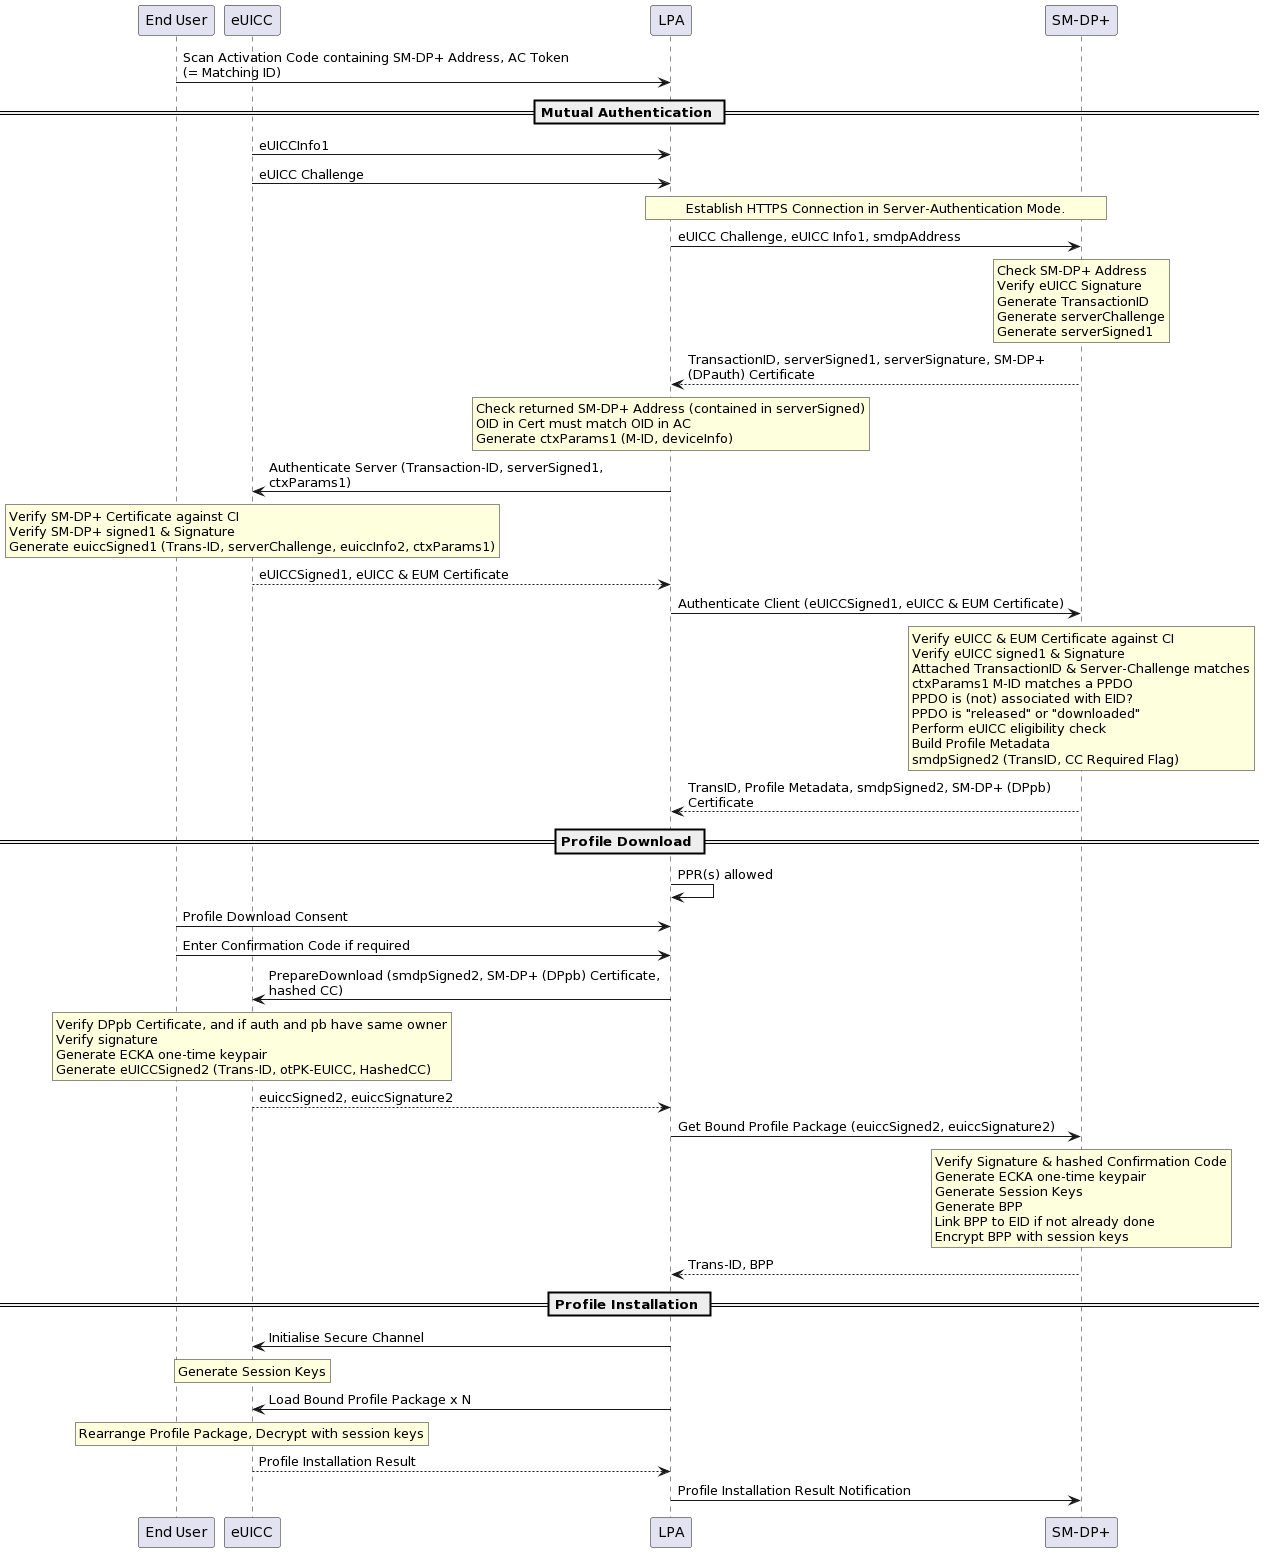
\includegraphics[width=.95\textwidth]{pictures/consumer_profile_download.png}
    \caption{Consumer Profile Download Procedure}
    \label{fig:ConMutAuth}
\end{figure}

The LPA requests eUICC information (eUICCInfo1 contains the supported SGP.22 version, supported CI PubKey Identifiers for signature verification and creation) and a eUICC Challenge. The function call [ES10b]GetEUICCChallenge is also the indication to the eUICC, that a new RSP session is starting. Only one session can be managed concurrently by the ISD-R. An additional call by the LPA should wait until the previously established RSP session is completed, but in the event, the eUICC will discard the previous context and may store the used keypair and SM-DP+ OID for future retry. The eUICC will then create a new context and generate a random 16-byte challenge.
The LPA will start a new HTTPS session with the SM-XX in "Server Authentication Mode" based on the input Address provided. The TLS session must use new keys (ECDHE as key establishment method) and the LPA verifies the SM-XX certificate (signature is valid and signed by GSMA CI or subordinate, Certificate (or any in trust chain) is not revoked or expired, and all the "critical" extensions defined are valid). \textit{However, regarding the expiry date and revocation, the LPA may not have any real-time knowledge or an up-to-date CRL, and therefore the verification may result in a false-positive!}
After a successful handshake, the LPA then initiates the mutual authentication of SM-XX and eUICC. The LPA sends the eUICC challenge, info and input SM-XX address to the SM-XX. SM-XX must verify, if it supports the requested spec-version and GSMA CI key to verify signatures and if the requested address matches it's own address \textit{why is this necessary? Integrity of the message?!}. If any of the verifications fail, the SM-XX will stop the execution and report an error code. Otherwise, the SM-XX then generates a TransactionID, which is used for every message of the remaining communication. Additionally a serverChallenge is generated and the SM-XX signs a package of the serverChallenge, received eUICC challenge and the transactionID with its private key. \textit{Communication between LPA and SM-XX is TLS-encrypted and therefore all communication between these parties is secure. The communication between LPA and eUICC however is not! \textbf{Attack of a malicious LPA which is the "Man in the middle"?!}} The LPA verifies, if the returned SM-XX address matches and generates a ctxParams1 object. (ctxParams1 contains the MatchingID and a list of device capabilites). The signed data is sent to the eUICC together with the SM-XX Certificate \textit{in clear}. The eUICC verifies the information on reception (in particular, if the eUICC challenge matches). In turn, the eUICC performs a signing operation over the received input data. eUICC ceritficate, EUM certificate and the signed data is sent over the LPA to SM-XX, which verifies this information again. Then, the eUICC and SM-XX are mutually authenticated to each other. The session continues depending on the operation.

\textit{A modification/replay of any of the messages between the LPA and SM-XX is prevented by TLS. The communication is secure, and known downgrade attacks on the TLS-Handshake are not possible, since the minimum supported version must be TLSv1.2, which is still considered secure (enough). However, one of the allowed cipher suites is  TLS\_ECDHE\_ECDSA\_WITH\_AES\_128\_CBC\_SHA256, which is considered weak based on the possible padding oracle attacks on CBC mode \url{https://security.stackexchange.com/questions/210072/why-does-ssl-labs-now-consider-cbc-suites-weak}. In theory, such an oracle attack could be possible, all functions on the ES9+ provide some output (error or success codes) when the input format is correct - and no output otherwise. The result would be to decrypt and read the communication between LPA and SM-XX. However, a more useful and feasible attack is, to sideload a malicious LPA, because then the communication is already in plain for the LPA. See \ref{chapter:LPA}. \\
Even if the TLS encryption is broken, all security relevant messages contain a signature of either the eUICC or the SM-XX, a transaction-ID of the current session and in the beginning, a challenge. The information might not be confidential anymore, but is still authentic and integrity protected.}


\subsubsection{Profile Installation}
Activation Code and Download - See below \ref{chapter:ProfMultiDevice}. 
    
Additionally, check for MitM attacks: In activation code, SM-DP+ URI \& AC\_Token is mandatory, but the SM-DP+ OID is optional (which would be verified later by the LPA). Could intercept the communication between Device and impersonate the SM-DP+. But need to forge a certificate issued by GSMA to gain trust of eUICC. Then download a malicious profile.
    
The installation is initiated by the LPA . The necessary information, SM-DP+ Address, MatchingID and possibly SM-DP+ OID is retrieved - either by entering an Activation Code, receiving an Event from SM-DS or on boot-up and reading the default SM-DP+. This data is used to perform the mutual authentication as described above with the MatchingID being the Activation Code Token, EventID or zero length respectively. If the SM-DP+-OID does not match the one read from the AC, the LPA must stop the procedure and inform the end user.

The SM-DP+ must verify, if there is a related pending profile download order in a "released" or "downloaded" state, and if it is linked to an EID, it does match the EID of the authenticated eUICC. The SM-DP+ performs an eligibility check for the target eUICC. If this check fails, the profile will be set into an "error" state, otherwise it checks, if the profile is already bound to an EID from a previous download attempt. \textit{There is a difference between "linked" to EID and "bound" to EID. If it is linked, the profile can only be installed on the eUICC with the target EID. If the profile package is already bound, it is encrypted and signed with the session keys relating to the EID from a previous download attempt.} If so, the binding is removed, and SM-DP+ generates a smdpSigned2 object (containing a flag, if a confirmation code is required, and an indication for the key used for protecting the profile). The transactionID, profile metadata, smdpSigned2 and profile package binding certificate of SM-DP+ (DPpb.ECDSA) is sent to the LPA. The LPA checks, if the profile metadata contains any PPR(s) (Disabling/Deletion not allowed) and if these PPR(s) are compatible with the current eUICC configuration. The profile download may be rejected at this stage.

If a confirmation code is required, the LPA asks the user to input this and hashes the code together with the current transaction ID (SHA256(SHA256(CC)|T-ID)). Then, the LPA asks the eUICC to prepare the profile download and sends the smdpSigned2, pb-Certificate and hash to the eUICC, which validates all information. If smdpSigned2 contains a valid key-identifier, the eUICC chooses this stored key for the RSP session. Otherwise it generates a new one-time ECKA key pair. The euiccSigned2 package contains the ot-public-key, hashed CC and again, the transaction-ID. Everything is returned to the LPA and SM-DP+. If the confirmation code was required, the SM-DP+ hashes the hashed CC stored alongside the profile with the Transaction ID (SHA256(H-CC|T-ID)) and compares the two values.

The SM-DP+ also generates a ot-ECKA key pair and session keys using the CRT (Control Reference Template), ot-PK of the eUICC and SM-DP+ ot-SK. The key-derivation process is based on SCP11a \parencite{GPC:AmendF} and results in a symmetric 128 bit AES key. These keys are either used to directly encrypt the profile package (make a PPP) and/or to bind the profile package (BPP) to the particular eUICC (SCP03t MACed and encrypted TLVs on how to initialise the secure channel, configure the ISD-P, profile protection keys, and the profile payload). The session keys are never transported, only information for the eUICC on how to generate them.

The BPP is sent to the LPA, which again verifies the profile metadata and contained PPRs. It segments the profile package, and sends the segments to the eUICC. eUICC generates the corresponding session keys to decrypt to profile package installation commands. 

\textit{The security between LPA and SM-DP+ is again ensured by TLS. As long as this session establishment (SM-DP+ is who is expected) is valid, the procedure is very secure, since every message has a transaction-ID and sensitive information (eUICC capabilities, certificates, profile metadata etc. is signed/MACed by the end parties). The LPA is therefore not able to modify any of this information during transit. In particular, the profile package is end-to-end encrypted, since SM-DP+ and eUICC generate an AES-Session Key based on the SCP11a standard, and use SCP03t as in the M2M Spec for profile package encryption.}



\subsubsection{SM-DS: Events, Notifications}
What is possible? Could events be crafted? How is the security? Is there any impact? DoS?

No authentication for registering events on SM-DS -> Any SM-DP+ is able to register a event for any EID

\subsubsection{On PKI and Certificate Structure}
Any certificate has a validation chain whose root is the GSMA CI certificate. 

\subsection{On Activation Code}
The Cleartext-Activation-Code possesses multiple risks for both the user and servers: 
\begin{itemize}
    \item The process of providing the AC to the End-User is out-of-spec. However, during transit, and since all the information is in clear-text, the SM-DP Address and OID could be modified by an attacker. The (naive) End-User then enters the "valid" AC in it's device and the download of a malicious profile starts. The EU must confirm the download from the server (and sees the name) but an attacker could easily present similar information. Still, the attackers SM-DP+ must have a valid GSMA certificate. But since the eUICC is not able to handle the revocation status of ALL certificates, the attacker could just reuse an old certificate of a previously valid server.
    \item M-ID can be modified/generated to try for a random profile download - or obtained through social engineering
    \item The confirmation-code-required flag is unnecessary in the AC. SM-DP+ knows, if the CC is required and will send it to the LPA anyway. If the Flag is set in the AC, the LPA must ask the user for inputting the CC, but the SM-DP+ may not expect this - this case is not defined. The confirmation code itself is a good 2FA method, but apparently rarely used in practice.
\end{itemize}

\subsection{LPA Security} \label{chapter:LPA}

What is an LPA? Application installed on device that handles the eUICC functionality.
Is a user/eSIM protected against the installation of a malicious LPA? Not necessarily. Some eSIMs/OS allow only signed LPAs, but most do not have this feature. 
Could this LPA handle unauthorized Profile Management? Could it be somehow secured? Is PIN Enforcement for user authentication an option? What are the possible actions of a malicious LPA?

\subsubsection{Profile Enabling, Disabling, Deletion} 
Everything done locally - could a malicious LPA do something?!
Absolutely, the LPA is in full control over the eSIM. On Android devices, the authenticity of the LPA is checked via a signature, an eSIM only allows commands from a known source. However, this feature is not found in the specification. Even so, many other OS (e.g. Windows or a custom IoT OS) allow any application to manage the eSIM. Therefore, a malicious LPA can often disable profiles or connectivity without user consent. 

As per specification:
User intent is required for profile enabling. This has to be ensured by the LPA. 

\subsubsection{Mutual Authentication}
During the Procedure of Mutual Authentication between the eUICC and SM-XX, the LPA acts as intermediary. It opens it's own TLS-Session between the LPA and SM-XX, but only in Server-Authentication Mode. A User could be prompted to download a new (but malicious) LPA (often done with naive users, sending a notification (SMS) informing about an "update" and providing a link, or through the Google Play Store for example). It is never checked by the eUICC (or servers), if the LPA is valid and trustworthy. The LPA could act as the MitM, providing either wrong information to the SM-XX or rerouting profile download information from the eUICC to the attackers SM-XX. 
This does not really apply to altering the information to the attackers advantage, since all the content is signed. But the LPA could craft completely new information and sign it with an available key.
In either case, it must provide information which is verifiable by the GSMA-CI, since both SM-XX and eUICC will go through their Chain-of-Trust. To gain such a certificate/key-pair, the attacker has to go through the certification process, similar as in M2M. But when presenting content to the eUICC, the attacker could also take advantage of revoked or outdated certificates, as the eUICC may not have the latest information.

\subsubsection{Device Lock-In}
A combination of a malicious LPA, the option to initiate profile downloads and PPRs allows an attacker to download a profile from his SM-DP+ server and install it on the eSIM. The security relies solely on a verifiable GSMA Certificate of the server. The profile download and enabling should require user consent, but this is ensured only by the LPA and no other factor, meaning it could be skipped by the malicious LPA or done in background.
There are two PPRs to set: Profile must not be disabled and profile must not be deleted. These PPRs are checked both by the LPA and eUICC. If an attacker downloads a profile with both these PPRs, the eUICC (and possibly attached device, since the eUICC is non-removable) is locked to the attacker, as the profile cannot be deleted. The gains for the attacker are similar to a ransomware attack. 
The only option for the User to disable the attackers profile is to perform a eSIM Memory Reset, which could be blocked by the mLPA.

\subsubsection{DDoS}
With enough devices with a malicious LPA installed, an attacker could create many "valid" session starts and profile downloads and occupy the SM-DP+. The attached eUICCs all have a default SM-DP+ and start the profile download procedure until the SM-DP+ becomes aware that no pending profile download exists.
\\
\textit{Fix/Improvement: Sign LPA Applications, allow only trusted applets via checks on OS level, add additional layer of trust by mutually authentication LPA to the server. \\ 
Add a strong 2FA authentication required for any profile management operation, e.g. SIM-PIN for confirmation.}

\subsection{One Profile on multiple Devices}\label{chapter:ProfMultiDevice}
Attack Idea in short: Download a valid profile on multiple devices and use it (not concurrently!) on all devices. At the end of the download procedure, the device must send a notification to the SM-DP+ about a successful profile download. Blocking this notification would allow the profile to be re-downloaded, as the SM-DP+ assumes the download failed. Could then download the profile on another device and use this profile on both devices (not at the same time, as the operator sees two devices with same IMSI attached concurrently to network and may block it then).

Process starts with the profile download initiation and ordering through operator. For the attack to work, the download through activation code (AC) is the only option, as all other options (Default SM-DP+ or SM-DS) require the EID either during the "DownloadOrder" or "ConfirmOrder" function.

Profile Download initation:
[ES2+]DownloadOrder: EID is optional. Profile state is set to "Allocated". Operator generates MatchingID for profile download.
[ES2+]ConfirmOrder: EID is optional. Profile state is set to "Released". MatchingID and SM-DP+ Address are provided to end-user via AC.

Common Mutual Authentication Procedure: Mutual Authentication between LPA and SM-DP+ involving the eUICC for challenge-response. EID is contained in the eUICC-Certificate, but it is not yet used for personalization of the profile! \textit{EID is part of the "subject" field of the eUICC certificate (organization=EUM, serialNumber=EID). The EID is extracted from the certificate in this step and kept at SM-DP+.}

Profile Download and Installation: AC and Confirmation Code is given to user. SM-DP+ must maintain a count of the number of attempts to download the profile and limit them accordingly. SM-DP+ and eUICC perform mutual authentication. SM-DP+ verifies, that pending profile download exists, and profile is in "released" or "downloaded" state. \textbf{"If this profile download order is already linked to an EID, verify that it matches the EID of the authenticated eUICC."} SM-DP+ performs "eligibility check" on the eUICC (needs to know EID for that, but EID is again not used to personalize the profile). User (based on consent) or LPA (based on PPRs) could reject the profile download at this stage - but at least user won't for the attack.

Download Confirmation: User has agreed to download the profile. LPA/eUICC checks the signature and certificate of SM-DP+, sends challenge and signature back. \textbf{"If the profile is not linked to the EID of the target eUICC, the SM-DP+ shall link the profile to the EID at this step."} Generates session keys and prepares BPP. Sends BPP to eUICC, sets profile to "downloaded" state.

Profile Installation: Procedure mostly between LPA and eUICC where LPA segments the profile package and sends it to eUICC. After a successful installation, the LPA sends notification to SM-DP+ about the status. This exact notification must be blocked to execute the attack. The profile state on the SM-DP+ then remains in "downloaded" and a download from another eUICC can be "retried" to have the same profile on multiple devices.
Notification Procedure: LPA sends notification about successful profile installation to SM-DP+. Each notification consists of a Sequence Number (against Replay), the profile installation result, recipient address, ICCID of the related profile and eUICC signature. "Each notification is sent on a best-effort basis" over a TLS-encrypted channel "when connectivity is available" \parencite{SGP:22}, meaning a blockade would go unnoticed. The SM-DP+ "shall" however confirm the reception of the notification - but it is never mentioned what happens if this confirmation is not received, which leads to the assumption of the LPA that everything is ok.

\textit{Assignment of the EID is done by the EUM and authority to issue certificates for each produced eUICC is also given to EUM. If an EUM assigns the identical EID to multiple eUICCs and issues the respective certificates for them (public key etc. can be completely valid and relate to the target eUICC, the only identical information must be the EID), the attack would work. SM-DP+ does check, if an EID is assigned to a PPDO. However, the only check about the EID itself is, if it does comply with the formatting. After the first download attempt, the EID is assigned to the PPDO and this PPDO can only be re-downloaded by the same EID (MatchingID is identical for multiple download retries). The eUICC does need to re-authenticate and a new ephemeral session key must be established to encrypt the profile, but (usually) the profile allows for re-binding (encryption of profile). Therefore, the download process should be possible with different public keys etc. as long as the EID remains identical and the profile download retry counter is not exceeded.
Another option is for the user to tell the operator the download has failed (when blocking the notification). The operator sees the profile in the "downloaded" state and may generate a new profile for the user on goodwill, even if the user has an operational profile on his device.}


\section{Comparison and assessment}
In this section, the similarities of the two systems should be compared and "rated".

E.g. both systems need to establish a secure channel to the server for profile download. M2M does this via symmetric keys, but still relies on certificates for authenticating each other. Consumer exclusively uses certificates and PKI for secure channels. Which way is better? Could M2M only use certificates, too?

Separation of SM-SR and SM-DP vs. SM-DP+

User initiated authentication

\textbf{The role of TLS in the system? Is it useful/required or is it more a "slap TLS on everything" approach?}
